\section{Lavoro svolto}
Il gruppo inizialmente ha deciso di adottare un metodo a cascata durante la stesura dei documenti iniziali e del way of working. 
Successivamente, con l'analisi dei requisiti e l'inizio della codifica, il gruppo ha adottato un metodo agile di tipo scrum al fine di organizzarsi meglio e preventivare in anticipo le attività da svolgere per raggiungere l'obiettivo prefissato.
Ogni sprint presenta le seguenti caratteristiche:
\begin{itemize}
    \item{Durata:} 2 settimane.
    \item{Attività svolte:} Attività che il gruppo si è prefissato e che ha portato a termine.
    \item{Difficoltà riscontrate:} A fine dello sprint, tramite un lavoro di retrospettiva si riflette sulle difficoltà incontrate.
    \item{Costi Previsti}
    \item{Costi Effettivi}
\end{itemize}

\subsection{Way of working}




\begin{longtable}{|c|c|}
    \hline
    \textbf{Legenda} & \\
    \hline
    RE & Responsabile \\
    \hline
    AN & Analista \\
    \hline
    VE & Verificatore \\
    \hline
    PR & Programmatore \\
    \hline
    PT & Progettista \\
    \hline
    AM & Amministratore \\
    \hline
\end{longtable}

\begin{longtable}{|p{0.085\textwidth}|c|c|c|c|c|c|c|}
    \hline
    Nome &\begin{tabular}[c]{@{}c@{}} dal 26/04\\ al 30/04 \end{tabular} & \begin{tabular}[c]{@{}c@{}}dal 01/05\\ al 04/05\end{tabular} & \begin{tabular}[c]{@{}c@{}}dal 04/05\\ al 12/05\end{tabular} & \begin{tabular}[c]{@{}c@{}}dal 13/05\\ al 19/05\end{tabular} & \begin{tabular}[c]{@{}c@{}}dal 20/05\\ al 26/05\end{tabular} & \begin{tabular}[c]{@{}c@{}}dal 27/5\\ al 03/06\end{tabular} & \begin{tabular}[c]{@{}c@{}}dal 04/06\\ al 09/06\end{tabular} \\
    \hline
    Ibra Elton & AN - 4 ore & VE - 2 ora& AN - 3 ore & RE - 3 ore & AN - 3 ore & VE -2 ore & PR - 4 ore  \\
    \hline
    Beschin Michele & AN - 3 ore & AN - 3 ore & RE - 4 ore & AN - 2 ore & VE - 2 ore & AN - 4 ore & PR - 3 ore  \\
    \hline
    Lotto Riccardo & AN - 3 ore & RE - 4 ore & AN - 3 ore & VE - 1 ore & AN - 4 ore & VE - 2 ore & PT - 3 ore\\
    \hline
    Bobirica Andrei Cristian & AN - 4 ore & AN - 3 ore & VE - 1 ore & AN - 2 ore & VE - 2 ore & AN - 4 ore & RE - 5 ore \\
    \hline
    Andreetto Alessio & AN - 3 ore & VE - 2 ore & AN - 3 ore & VE - 2 ore & AN - 4 ore & RE - 4 ore & AN - 3 ore \\
    \hline
    Corbu Teodor Mihail & AN - 3 ore & AN - 4 ore & VE - 2 ore & AN - 2 ore & RE - 3 ore & AN - 3 ore & VE - 2 ore\\
    \hline
    Ore settimanali & 20 &  18&  16&  12&  18&  19&  20 \\
    \hline 
    Costi preventivati & 525 € & 400 € & 430 € & 285 € & 470 € & 495 € & 470 € \\
    \hline
    Costi effettivi &  500 €& 450 € & 405 € & 300 €& 445 € & 475 € & 445 € \\
    \hline
\end{longtable}






\subsection{Requirements and technology baseline}
In vista della prima revisione RTB, il gruppo ha scelto di cambiare metodologia di lavoro. Per facilitare la stesura del codice, si è scelto di optare per una metodologia agile suddivisa in sprint.


\subsubsection{Sprint 1}
\begin{center}
    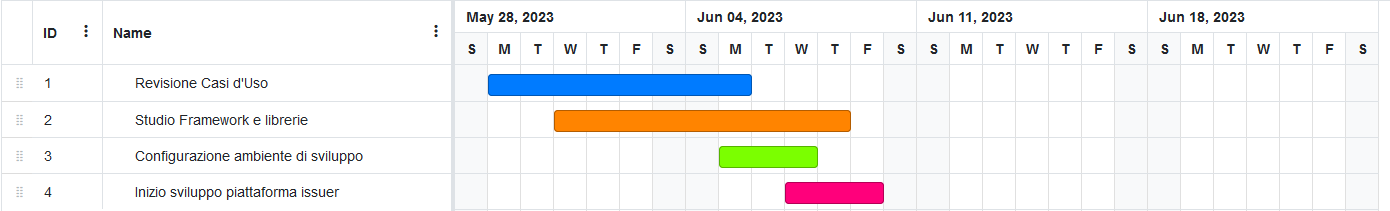
\includegraphics[scale = 0.4]{./res/img/Sprint_1.png}
  \end{center}

\begin{itemize}
\item \textbf{Durata:} 29/05/2023 - 09/06/2023 
\item \textbf{Attività svolte:}
\begin{itemize}
    \item Ampliamento e revisione della sezione "casi d'uso" all'interno del documento \AdRdocumento;
    \item Analisi e studio dei framework e librerie da utilizzare per lo sviluppo del codice;
    \item Creazione e configurazione dell'ambiente di sviluppo;
    \item Inizio sviluppo piattaforma issuer.
\end{itemize}
\item \textbf{Difficoltà riscontrate:}
\begin{itemize}
    \item Lo sviluppo della piattaforma holder non era compatibile parallelamente a quella issuer; 
    \item Difficoltà nel gestire tutte le istanze all'interno di Docker\glo, si è optato per mantenere su container docker soltanto le API.
\end{itemize}
\newpage
\item \textbf{Costi Previsti:}
\begin{longtable}{|c|c|c|c|}
    \hline
    Ruolo & Descrizione & Ore & Costo \\
    \hline
    RE & Responsabile & 5 & 150€ \\
    \hline
    AN & Analista & 5 & 125€ \\
    \hline
    VE & Verificatore & 5 & 100€ \\
    \hline
    PR & Programmatore & 8 & 120€ \\
    \hline
    PT & Progettista & 4 & 100€ \\
    \hline
    AM & Amministratore & 3 & 60€ \\
    \hline
    Totale & & 30 & 655€ \\
    \hline
    \end{longtable}
\item \textbf{Costi effettivi:}
\begin{longtable}{|p{0.1\textwidth}|c|c|c|c|c|c|c|c|}
    \hline
    Nome & RE & AN & VE & PR & PT & AM & Ore & Costi\\
    \hline
    Ibra Elton &5 & & & & & &5 & 150€\\
    \hline
    Beschin Michele & & & &4 & & &4 & 60€ \\
    \hline
    Lotto \newline  Riccardo & & & &5 & & &5& 75€ \\
    \hline
    Bobirica Andrei Cristian & & & & &3 &2 &5 & 115€\\
    \hline
    Andreetto Alessio & &6 & & & & &6 & 150€\\
    \hline
    Corbu Teodor Mihail & & &6 & & & &6 & 120€\\
    \hline
    Totale &5 &6 &6 &9 &3 &2 &31& 670€\\
    \hline
\end{longtable}
\end{itemize}

\subsubsection{Sprint 2}
\begin{center}
    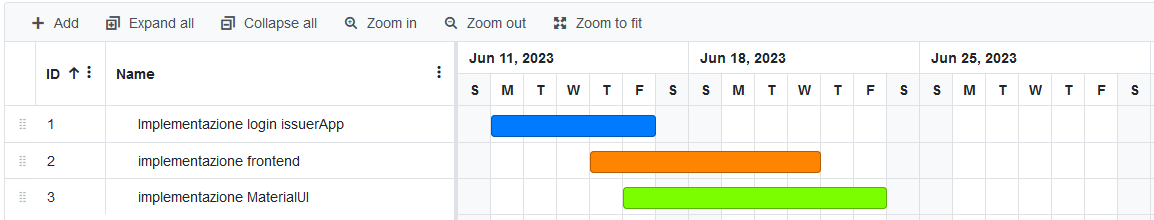
\includegraphics[scale = 0.45]{./res/img/Sprint_2.png}
  \end{center}

\begin{itemize}
    \item \textbf{Durata:} 12/06/2023 - 23/06/2023 
    \item \textbf{Attività svolte:}
    \begin{itemize}
        \item È stata implementata la libreria grafica Material UI su un branch separato;
        \item È stato implementato il sistema di login per issuer app; 
        \item Implementazione del front-end per la richiesta di credenziale nell'issuer.
    \end{itemize}
    \item \textbf{Difficoltà riscontrate:}
    \begin{itemize}
        \item Al momento attuale lo sviluppo del verifier non è compatibile parallelamente ad issuer.
    \end{itemize}
    \item \textbf{Costi Previsti:}
    \begin{longtable}{|c|c|c|c|}
        \hline
        Ruolo & Descrizione & Ore & Costo \\
        \hline
        RE & Responsabile & 4 & 120€ \\
        \hline
        AN & Analista & 0 & 0€ \\
        \hline
        VE & Verificatore & 3 & 60€ \\
        \hline
        PR & Programmatore & 13 & 195€ \\
        \hline
        PT & Progettista & 15 & 375€ \\
        \hline
        AM & Amministratore & 4 & 80€ \\
        \hline
        Totale & & 39 & 830€ \\
        \hline
        \end{longtable}
    \item \textbf{Costi effettivi:}
    \begin{longtable}{|p{0.1\textwidth}|c|c|c|c|c|c|c|c|}
        \hline
        Nome & RE & AN & VE & PR & PT & AM & Ore & Costi\\
        \hline
        Ibra \newline Elton & & & &6 & & &6 & 90€\\
        \hline
        Beschin Michele & & & & &7 & &7 & 175€\\
        \hline
        Lotto \newline Riccardo &2 & & & &5 & &7 & 185€\\
        \hline
        Bobirica Andrei Cristian & & & & &3 &4 &7 & 155€\\
        \hline
        Andreetto Alessio &2 & & &3 & & &5 & 105€\\
        \hline
        Corbu Teodor Mihail & & &3 &4 & & &7 & 120€\\
        \hline
        Totale &4 &0 &3 &13 &15 &4 &39 & 830€\\
 
        \hline
    \end{longtable}
    \end{itemize}

\subsubsection{Sprint 3}
\begin{center}
    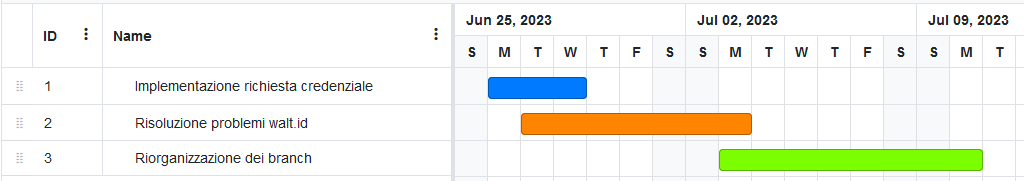
\includegraphics[scale = 0.5]{./res/img/Sprint_3.png}
  \end{center}
\begin{itemize}
    \item \textbf{Durata:} 26/06/2023 - 07/07/2023 
    \newpage
    \item \textbf{Attività svolte:}
    \begin{itemize}
        \item Risolto alcuni problemi riscontrati nello sprint precedente con la libreria walt id;
        \item Organizzato i branch nella repository github.
    \end{itemize}
    \item \textbf{Difficoltà riscontrate:}
    \begin{itemize}
        \item In vista del PoC abbiamo sperimentato l’utilizzo della libreria walt.id per la generazione di credenziali
        abbiamo riscontrato delle problematiche riguardanti bug/mancanza di documentazione/parti di funzionalità non complete.
    \end{itemize}
    \item \textbf{Costi Previsti:}
    \begin{longtable}{|c|c|c|c|}
        \hline
        Ruolo & Descrizione & Ore & Costo \\
        \hline
        RE & Responsabile & 1 & 30€ \\
        \hline
        AN & Analista & 1 & 25€ \\
        \hline
        VE & Verificatore & 2 & 40€ \\
        \hline
        PR & Programmatore & 3 & 45€ \\
        \hline
        PT & Progettista & 1 & 25€ \\
        \hline
        AM & Amministratore & 2 & 40€ \\
        \hline
        Totale & & 14 & 350€ \\
        \hline
        \end{longtable}
        
        
    \item \textbf{Costi effettivi:}
    \begin{longtable}{|p{0.1\textwidth}|c|c|c|c|c|c|c|c|c|}
        \hline
        Nome & RE & AN & VE & PR & PT & AM & Ore & Costi\\
        \hline
        Ibra \newline Elton & & & &3 & & &3 & 45€\\
        \hline
        Beschin Michele & & & & & &3 &3 & 60€\\
        \hline
        Lotto \newline Riccardo & & &2 &1 & & &3 & 55€\\
        \hline
        Bobirica Andrei Cristian & & &1 &2 & & &3 &  50€\\
        \hline
        Andreetto Alessio &2 &2 & & & & &4 & 110€\\
        \hline
        Corbu Teodor Mihail & & & & &3 & &3 & 75€\\
        \hline
        Totale &2 &2 &3 &6 &3 &3 &19 & 395€\\
        \hline
    \end{longtable}
    \end{itemize}

\subsubsection{Sprint 4}
\begin{center}
    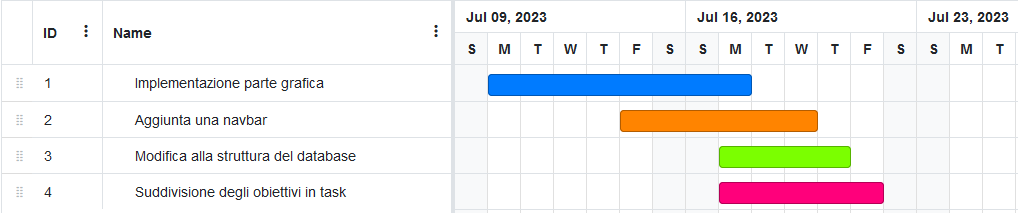
\includegraphics[scale = 0.5]{./res/img/Sprint_4.png}
  \end{center}
\begin{itemize}
    \item \textbf{Durata:} 10/07/2023 - 21/07/2023 
    \item \textbf{Attività svolte:}
    \begin{itemize}
        \item La parte grafica prima implementata su un branch a parte è stata implementata anche sull'applicativo issuer;
        \item Assieme alla parte grafica è stata aggiunta una navbar nell'applicativo issuer; 
        \item Il database ha subito delle modifiche in particolare alcuni campi oltre che cambiare nome hanno cambiato valori registrati;
        \item I macro obiettivi che volevamo raggiungere sono stati suddivisi in task più piccoli da gestire per il gruppo e per i componenti singoli.
    \end{itemize}
    \item \textbf{Difficoltà riscontrate:}
    \item \textbf{Costi Previsti:}
    \begin{longtable}{|c|c|c|c|}
        \hline
        Ruolo & Descrizione & Ore & Costo \\
        \hline
        RE & Responsabile & 2 & 60€ \\
        \hline
        AN & Analista & 2 & 50€ \\
        \hline
        VE & Verificatore & 2 & 40€ \\
        \hline
        PR & Programmatore & 16 & 240€ \\
        \hline
        PT & Progettista & 8 & 200€ \\
        \hline
        AM & Amministratore & 8 & 160€ \\
        \hline
        Totale & & 38 & 750€ \\
        \hline
        \end{longtable}
    \item \textbf{Costi effettivi:}
    \begin{longtable}{|p{0.1\textwidth}|c|c|c|c|c|c|c|c|}
        \hline
        Nome & RE & AN & VE & PR & PT & AM & Ore & Costi\\
        \hline
        Ibra \newline Elton & &2 & &3 &3 & &8 & 170€\\
        \hline
        Beschin Michele &2 & & &5 & & &7 & 135€\\
        \hline
        Lotto \newline Riccardo & & &3 &4 & & &7 & 120€\\
        \hline
        Bobirica Andrei Cristian & & & &5 & & &5 & 75€\\
        \hline
        Andreetto Alessio & &1 & & &5 & &6 & 150€\\
        \hline
        Corbu Teodor Mihail & & & & & &7 &7 & 140€\\
        \hline
        Totale &2 &3 &3 &17 &8 &7 &40 & 790€\\
        \hline
    \end{longtable}
    \end{itemize}

    \subsubsection{Sprint 5}
\begin{center}
    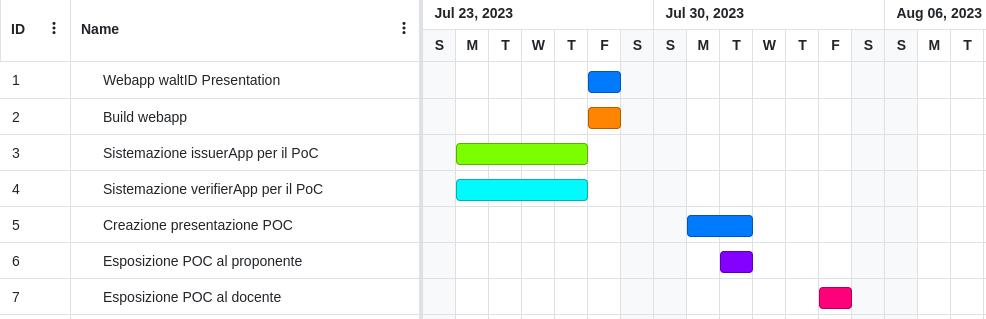
\includegraphics[scale = 0.5]{./res/img/Sprint 5.png}
  \end{center}
\begin{itemize}
    \item \textbf{Durata:} 24/07/2023 - 04/08/2023 
    \item \textbf{Attività svolte:}
    \begin{itemize}
        \item Build delle webApp
        \item Deploy su Docker e creazione container Apache e Node.js per le webApp e backend
        \item Creazione release POC 
    \end{itemize}
    \item \textbf{Difficoltà riscontrate:}
    \begin{itemize}
        \item Configurare Apache per utilizzo di webapp sviluppate con react
    \end{itemize}
    \item \textbf{Costi Previsti:}
    \begin{longtable}{|c|c|c|c|}
        \hline
        Ruolo & Descrizione & Ore & Costo \\
        \hline
        RE & Responsabile & 9 &  270€\\
        \hline
        AN & Analista & 2 &  50€\\
        \hline
        VE & Verificatore &  7 &  140€\\
        \hline
        PR & Programmatore & 8 &  120€\\
        \hline
        PT & Progettista & 20 &  300€\\
        \hline
        AM & Amministratore & 11 & 220€ \\
        \hline
        Totale & &  57&  1100€\\
        \hline
        \end{longtable}
    \item \textbf{Costi effettivi:}
    \begin{longtable}{|p{0.1\textwidth}|c|c|c|c|c|c|c|c|}
        \hline
        Nome & RE & AN & VE & PR & PT & AM & Ore & Costi\\
        \hline
        Ibra \newline Elton & & & & & & & & \\
        \hline
        Beschin Michele & & & & & & & & \\
        \hline
        Lotto \newline Riccardo & & & & & & & & \\
        \hline
        Bobirica Andrei Cristian & & & & & & & & \\
        \hline
        Andreetto Alessio & & & & & & & & \\
        \hline
        Corbu Teodor Mihail & & & & & & & & \\
        \hline
        Totale & & & & & & & & \\
        \hline
    \end{longtable}
    \end{itemize}

    \subsubsection{Sprint 6}
    \begin{center}
        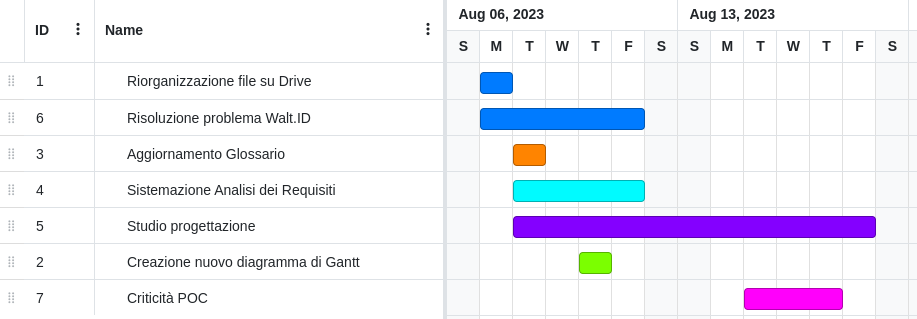
\includegraphics[scale = 0.5]{./res/img/Sprint 6.png}
      \end{center}
    \begin{itemize}
        \item \textbf{Durata:} 07/08/2023 - 18/08/2023 
        \item \textbf{Attività svolte:}
        \begin{itemize}
            \item Creazione presentazione e incontro con il docente Cardin
            \item Creazione presentazione e incontro con il docente Vardanega
            \item Riorganizzazione dei file su Drive e creazione di un nuovo diagramma di Gantt
            \item Aggiornamento glossario
            \item Risoluzione di alcuni problemi nel documento Analisi dei Requisiti
            \item Ricerca riguardo le tecnologie utilizzate
            \item Studio progettazione
            \item Credential Issuing
            \item Ricerca sui test automatici
            
        \end{itemize}
        \item \textbf{Difficoltà riscontrate:}
        \begin{itemize}
            \item Incompatibilità con i software waltID kit (SSI kit, IDP kit) causa incompletezza e mancanza documentazione.
        \end{itemize}
        \item \textbf{Costi Previsti:}
        \begin{longtable}{|c|c|c|c|}
            \hline
            Ruolo & Descrizione & Ore & Costo \\
            \hline
            RE & Responsabile & 9 & 270€\\
            \hline
            AN & Analista & 3 &  75€\\
            \hline
            VE & Verificatore & 7 &  140€\\
            \hline
            PR & Programmatore & 10 & 150€ \\
            \hline
            PT & Progettista & 25 &  625€\\
            \hline
            AM & Amministratore & 11 &  220€\\
            \hline
            Totale & &  65&  1480€\\
            \hline
            \end{longtable}
        \item \textbf{Costi effettivi:}
        \begin{longtable}{|p{0.1\textwidth}|c|c|c|c|c|c|c|c|}
            \hline
            Nome & RE & AN & VE & PR & PT & AM & Ore & Costi\\
            \hline
            Ibra \newline Elton & & & & & & & & \\
            \hline
            Beschin Michele & & & & & & & & \\
            \hline
            Lotto \newline Riccardo & & & & & & & & \\
            \hline
            Bobirica Andrei Cristian & & & & & & & & \\
            \hline
            Andreetto Alessio & & & & & & & & \\
            \hline
            Corbu Teodor Mihail & & & & & & & & \\
            \hline
            Totale & & & & & & & & \\
            \hline
        \end{longtable}
        \end{itemize}

        \subsubsection{Sprint 7}
        \begin{center}
            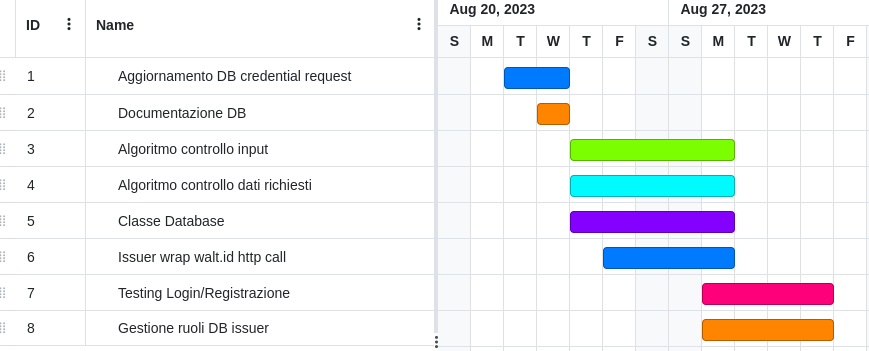
\includegraphics[scale = 0.5]{./res/img/Sprint 7.png}
          \end{center}
        \begin{itemize}
            \item \textbf{Durata:} 21/08/2023 - 01/09/2023 
            \item \textbf{Attività svolte:}
            \begin{itemize}
                \item Implementazione Verifiable Presentation e Walt.Id
                \item Diagrammi ER
                \item Implementazione database
                \item Inizio documento Specifica Tecnica
                \item Finita implementazione classe database nel back-end
                \item Finita implementazione endpoint back-end issuer
                \item Implementati algoritmi di controllo
                \item Implementato front-end issuer
                
                
            \end{itemize}
            \item \textbf{Difficoltà riscontrate:}
             \begin{itemize}
                \item  Data l'incompatibilità dei kit precedenti abbiamo avuto la necessità di trovare un nuovo kit di WaltId per procedere. Il kit da noi trovato e compatibile per l'issuing e presentazione della credenziale non risulta documentato.
             \end{itemize}
            \item \textbf{Costi Previsti:}
            \begin{longtable}{|c|c|c|c|}
                \hline
                Ruolo & Descrizione & Ore & Costo \\
                \hline
                RE & Responsabile & 8 &  240€\\
                \hline
                AN & Analista & 3 &  75€\\
                \hline
                VE & Verificatore & 7 & 140€ \\
                \hline
                PR & Programmatore & 10 &  150€\\
                \hline
                PT & Progettista & 15 &  375€\\
                \hline
                AM & Amministratore & 10 &  200€\\
                \hline
                Totale & &  53 &  1180€\\
                \hline
                \end{longtable}
            \item \textbf{Costi effettivi:}
            \begin{longtable}{|p{0.1\textwidth}|c|c|c|c|c|c|c|c|}
                \hline
                Nome & RE & AN & VE & PR & PT & AM & Ore & Costi\\
                \hline
                Ibra \newline Elton & & & & & & & & \\
                \hline
                Beschin Michele & & & & & & & & \\
                \hline
                Lotto \newline Riccardo & & & & & & & & \\
                \hline
                Bobirica Andrei Cristian & & & & & & & & \\
                \hline
                Andreetto Alessio & & & & & & & & \\
                \hline
                Corbu Teodor Mihail & & & & & & & & \\
                \hline
                Totale & & & & & & & & \\
                \hline
            \end{longtable}
            \end{itemize}


        \subsubsection{Sprint 8}
        \begin{center}
            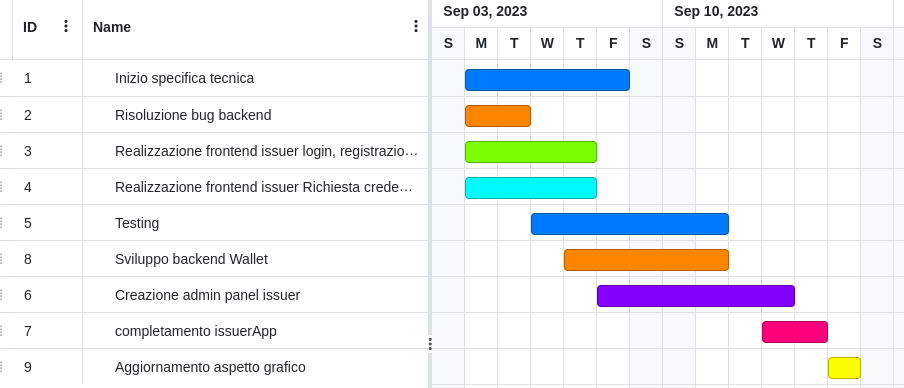
\includegraphics[scale = 0.5]{./res/img/Sprint 8.png}
          \end{center}
        \begin{itemize}
            \item \textbf{Durata:} 04/08/2023 - 15/09/2023 
            \item \textbf{Attività svolte:}
            \begin{itemize}
                \item Finita implementazione del front-end dell’issuerApp
                \item Notevole estensione del documento Specifica Tecnica
                \item Finita implementazione Pattern Data Strategy, Routing e Data Scrapper nell’issuerApp
                \item Completato l’issuerApp 
                \item inizio backend wallet
                \item stesura del verbale dopo la chiamata con l’azienda
                
            \end{itemize}
            \item \textbf{Difficoltà riscontrate:}
            \item \textbf{Costi Previsti:}
            \begin{longtable}{|c|c|c|c|}
                \hline
                Ruolo & Descrizione & Ore & Costo \\
                \hline
                RE & Responsabile & 8 &  240€\\
                \hline
                AN & Analista & 6 &  150€\\
                \hline
                VE & Verificatore & 14 &  280€\\
                \hline
                PR & Programmatore & 20 & 300€ \\
                \hline
                PT & Progettista & 15 & 375€ \\
                \hline
                AM & Amministratore & 6 &  120€\\
                \hline
                Totale & & 69 & 1465€ \\
                \hline
                \end{longtable}
            \item \textbf{Costi effettivi:}
            \begin{longtable}{|p{0.1\textwidth}|c|c|c|c|c|c|c|c|}
                \hline
                Nome & RE & AN & VE & PR & PT & AM & Ore & Costi\\
                \hline
                Ibra \newline Elton & & & & & & & & \\
                \hline
                Beschin Michele & & & & & & & & \\
                \hline
                Lotto \newline Riccardo & & & & & & & & \\
                \hline
                Bobirica Andrei Cristian & & & & & & & & \\
                \hline
                Andreetto Alessio & & & & & & & & \\
                \hline
                Corbu Teodor Mihail & & & & & & & & \\
                \hline
                Totale & & & & & & & & \\
                \hline
            \end{longtable}
            \end{itemize}


        \subsubsection{Sprint 9}
        \begin{center}
            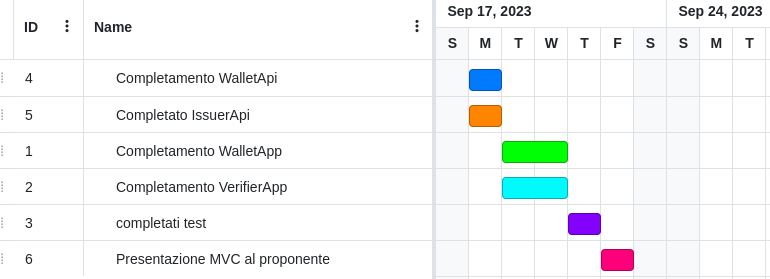
\includegraphics[scale = 0.5]{./res/img/Sprint 9.png}
          \end{center}
        \begin{itemize}
            \item \textbf{Durata:} 18/09/2023 - 29/09/2023 
            \item \textbf{Attività svolte:}
            \begin{itemize}
                \item Completato walletApp
                \item Completato verifierApp
                \item Completato testing delle 3 webapp 
                
            \end{itemize}
            \item \textbf{Difficoltà riscontrate:}
            \begin{itemize}
                \item Difficoltà riscontrata nell'utilizzo della libreria di testing. 
            \end{itemize}
            \item \textbf{Costi Previsti:}
            \begin{longtable}{|c|c|c|c|}
                \hline
                Ruolo & Descrizione & Ore & Costo \\
                \hline
                RE & Responsabile & 8 & 240€\\
                \hline
                AN & Analista & 7 &  175€\\
                \hline
                VE & Verificatore & 14 & 280€ \\
                \hline
                PR & Programmatore & 20 &  300€\\
                \hline
                PT & Progettista & 13 & 325€ \\
                \hline
                AM & Amministratore & 6 & 120€ \\
                \hline
                Totale & & 68 & 1440€ \\
                \hline
                \end{longtable}
            \item \textbf{Costi effettivi:}
            \begin{longtable}{|p{0.1\textwidth}|c|c|c|c|c|c|c|c|}
                \hline
                Nome & RE & AN & VE & PR & PT & AM & Ore & Costi\\
                \hline
                Ibra \newline Elton & & & & & & & & \\
                \hline
                Beschin Michele & & & & & & & & \\
                \hline
                Lotto \newline Riccardo & & & & & & & & \\
                \hline
                Bobirica Andrei Cristian & & & & & & & & \\
                \hline
                Andreetto Alessio & & & & & & & & \\
                \hline
                Corbu Teodor Mihail & & & & & & & & \\
                \hline
                Totale & & & & & & & & \\
                \hline
            \end{longtable}
            \end{itemize}